\section*{Chapitre 20 - Solides de l'espace}
 \addcontentsline{toc}{section}{Chapitre 20 - Solides de l'espace}
\subsection*{I. Reconnaître les solides usuels}
 \addcontentsline{toc}{subsection}{I. Reconnaître les solides usuels}


\begin{center}

\newcolumntype{C}[1]{>{\centering\arraybackslash}p{#1}}

\arrayrulecolor{Couleur8}

\begin{tabular}{|C{2.15cm}|C{2.15cm}|C{2.15cm}|C{2.15cm}|C{2.15cm}|C{2.15cm}|C{2.15cm}|}

\hline

\cellcolor{Couleur8!25} & \cellcolor{Couleur8!25} & \cellcolor{Couleur8!25}  & \cellcolor{Couleur8!25} & \cellcolor{Couleur8!25} & \cellcolor{Couleur8!25}& \cellcolor{Couleur8!25} \\

\hline

\rule{0pt}{2.5cm}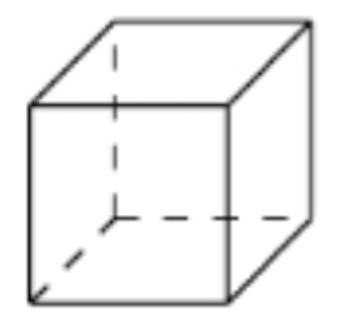
\includegraphics[scale=.35]{IMG/11} & 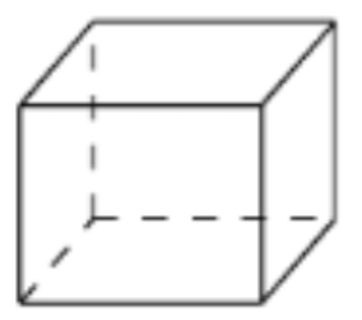
\includegraphics[scale=.35]{IMG/12} & 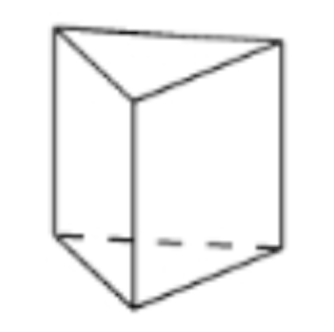
\includegraphics[scale=.32]{IMG/13} & 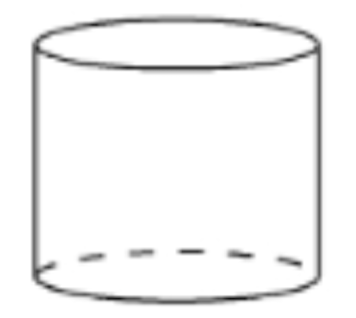
\includegraphics[scale=.35]{IMG/14} & 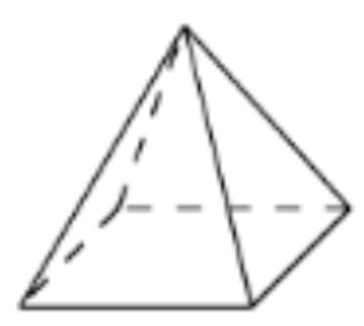
\includegraphics[scale=.33]{IMG/15} & 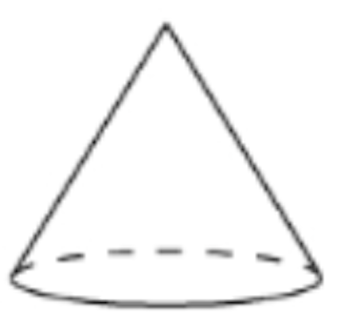
\includegraphics[scale=.34]{IMG/16}& 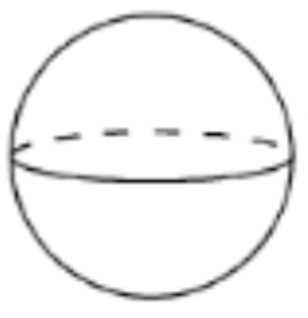
\includegraphics[scale=.35]{IMG/17}\\

\hline

\end{tabular}


\end{center}


\vspace{1cm}


\begin{Exemple}

\begin{minipage}[c]{.5\textwidth}

\begin{center}
\begin{tikzpicture}[scale=1.2]
% Cube en perspective cavalière
\fill[Couleur7!75] (0,0) rectangle (1.5,1.5);
\fill[Couleur11!75] (1.5,1.5) -- (2.2,2.2) -- (2.2,0.7) -- (1.5,0) -- cycle;
\fill[Couleur8!75] (0,1.5) -- (0.7,2.2) -- (2.2,2.2) -- (1.5,1.5) -- cycle;

% Contours
\draw[thick] (0,0) rectangle (1.5,1.5);
\draw[thick] (1.5,1.5) -- (2.2,2.2) -- (2.2,0.7) -- (1.5,0);
\draw[thick] (0,1.5) -- (0.7,2.2) -- (2.2,2.2);
\draw[thick, dashed] (0,0) -- (0.7,0.7) -- (0.7,2.2);
\draw[thick, dashed] (0.7,0.7) -- (2.2,0.7);
\end{tikzpicture} \\
\textbf{Représentation en perspective \\
cavalière d'un cube }
\end{center}
\end{minipage}
\hfill
\begin{minipage}[c]{.5\textwidth}
\begin{center}
\begin{tikzpicture}[scale=0.8]
\def\cote{2}

% Face centrale
\draw[thick,fill=Couleur7!75] (\cote,\cote) rectangle (2*\cote,2*\cote);
\node at (1.5*\cote,1.5*\cote) {Face};

% Face du haut
\draw[thick,fill=Couleur8!75] (\cote,2*\cote) rectangle (2*\cote,3*\cote);
\node at (1.5*\cote,2.5*\cote) {Haut};

% Face de gauche
\draw[thick,fill=Couleur12!75] (0,\cote) rectangle (\cote,2*\cote);
\node at (0.5*\cote,1.5*\cote) {Gauche};

% Face de droite
\draw[thick,fill=Couleur11!75] (2*\cote,\cote) rectangle (3*\cote,2*\cote);
\node at (2.5*\cote,1.5*\cote) {Droite};

% Face du bas
\draw[thick,fill=Couleur9!75] (\cote,0) rectangle (2*\cote,\cote);
\node at (1.5*\cote,0.5*\cote) {Bas};

% Face arrière
\draw[thick,fill=Couleur6!75] (\cote,3*\cote) rectangle (2*\cote,4*\cote);
\node at (1.5*\cote,3.5*\cote) {Arrière};



\end{tikzpicture}

\textbf{Patron d'un cube }

\end{center}
\end{minipage}

\end{Exemple}

\vspace{1cm}

\begin{Exemple}
\begin{minipage}[c]{.5\textwidth}
\begin{center}

\begin{tikzpicture}[scale=0.8]

% Dimensions du pavé droit (mêmes que le patron)
\def\longueur{4}
\def\largeur{2.5}  
\def\hauteur{1.5}

% Angle et facteur de réduction pour la perspective cavalière
\def\angle{30}
\def\facteur{0.5}

% Calcul des décalages pour la profondeur
\pgfmathsetmacro{\dx}{\largeur*\facteur*cos(\angle)}
\pgfmathsetmacro{\dy}{\largeur*\facteur*sin(\angle)}
% Face arrière (partiellement visible)
\draw[thick] (\dx,\dy) rectangle (\longueur+\dx,\hauteur+\dy);

% Face avant (visible)
\draw[thick,fill=Couleur7!60] (0,0) rectangle (\longueur,\hauteur);



% Arêtes reliant avant et arrière

\draw[thick] (\longueur,0) -- (\longueur+\dx,\dy);
\draw[thick] (0,\hauteur) -- (\dx,\hauteur+\dy);
\draw[thick] (\longueur,\hauteur) -- (\longueur+\dx,\hauteur+\dy);

% Face du dessus (visible)
\draw[thick,fill=Couleur8!60] (0,\hauteur) -- (\dx,\hauteur+\dy) -- (\longueur+\dx,\hauteur+\dy) -- (\longueur,\hauteur) -- cycle;

% Face de droite (visible)
\draw[thick,fill=Couleur12!60] (\longueur,0) -- (\longueur+\dx,\dy) -- (\longueur+\dx,\hauteur+\dy) -- (\longueur,\hauteur) -- cycle;

% Arêtes cachées en pointillés
\draw[thick,dashed, black] (0,0) -- (\dx,\dy);
\draw[thick,dashed, black] (\dx,\dy) -- (\dx,\hauteur+\dy);
\draw[thick,dashed, black] (\dx,\dy) -- (\longueur+\dx,\dy);

\end{tikzpicture}\\
\textbf{Représentation en perspective \\
cavalière d'un pavé droit }
\end{center}
\end{minipage}
\hfill
\begin{minipage}[c]{.5\textwidth}
\begin{center}
\begin{tikzpicture}[scale=0.6]
% Dimensions du pavé droit
\def\longueur{4}
\def\largeur{2.5}
\def\hauteur{1.5}

% Face avant (longueur × hauteur)
\draw[fill=Couleur7!60] (0,0) rectangle (\longueur,\hauteur);
\node at (0.5*\longueur,0.5*\hauteur) {Face};

% Face arrière (longueur × hauteur)
\draw[fill=Couleur6!60] (0,\hauteur+\largeur) rectangle (\longueur,\hauteur+\largeur+\hauteur);
\node at (0.5*\longueur,\hauteur+\largeur+0.5*\hauteur) {Arrière};

% Face gauche (largeur × hauteur)
\draw[fill=Couleur12!60] (-\largeur,0) rectangle (0,\hauteur);
\node at (-0.5*\largeur,0.5*\hauteur) {{Gauche}};

% Face droite (largeur × hauteur)
\draw[fill=Couleur11!60] (\longueur,0) rectangle (\longueur+\largeur,\hauteur);
\node at (\longueur+0.5*\largeur,0.5*\hauteur) {{Droite}};

% Face bas (longueur × largeur)
\draw[fill=Couleur9!60] (0,-\largeur) rectangle (\longueur,0);
\node at (0.5*\longueur,-0.5*\largeur) {Bas};

% Face haut (longueur × largeur)
\draw[fill=Couleur8!60] (0,\hauteur) rectangle (\longueur,\hauteur+\largeur);
\node at (0.5*\longueur,\hauteur+0.5*\largeur) {Haut};




\end{tikzpicture} \\
% Patron de pavé droit
\textbf{Patron d'un pavé droit}
\end{center}
\end{minipage}

\end{Exemple}


\newpage 


\subsection*{II. Représentation dans l'espace}
 \addcontentsline{toc}{subsection}{II. Représentation dans l'espace}
\begin{Exemple}
\begin{minipage}[c]{.5\textwidth}

On considère l'assemblage de cubes suivant. \\
Le but est d'identifier les vues de face, de dessus, de droite et de gauche de cet assemblage de cubes.
\begin{center}

\includegraphics[scale=0.5]{IMG/2}
\end{center}
\end{minipage} \hfill \begin{minipage}[c]{.5\textwidth}

\begin{center}
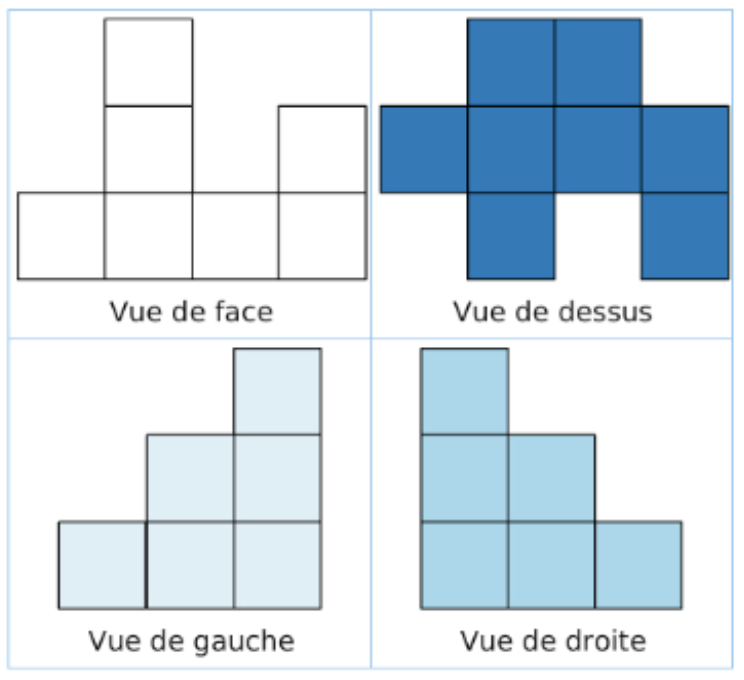
\includegraphics[scale=0.5]{IMG/3}
\end{center}

\end{minipage}

\end{Exemple}



\subsection*{III. Les volumes}
 \addcontentsline{toc}{subsection}{III. Les volumes}

\begin{Définition}
Le volume d'un solide est une grandeur correspondant à la place que l'objet occupe dans l'espace.
\end{Définition}


\begin{Définition}
Le centimètre cube est une unité de volume. On la note cm$^3$.  \\
1 cm$^3$ est le volume d'un cube d'arête 1 cm.
\end{Définition}

\begin{center}
\begin{tikzpicture}

 % Troisième ligne - noms des positions
\node[draw, Couleur8!50,fill=Couleur8!15, minimum width=2.3cm, minimum height=0.9cm, align=center] at (-2,0.85) {km³};
\node[draw, Couleur8!50, fill=Couleur8!15,minimum width=2.3cm, minimum height=0.9cm, align=center] at (0.3,0.85) {hm³};
\node[draw, Couleur8!50, fill=Couleur8!15,minimum width=2.3cm, minimum height=0.9cm, align=center] at (2.6,0.85) {dam³};
\node[draw, Couleur8, fill=Couleur8!45,minimum width=2.3cm, minimum height=0.9cm, align=center] at (4.9,0.85) {m³};
\node[draw,Couleur8!75, fill=Couleur8!35,minimum width=2.3cm, minimum height=0.9cm, align=center] at (7.2,0.85) {dm³};
\node[draw, Couleur8!75, fill=Couleur8!35,minimum width=2.3cm, minimum height=0.9cm, align=center] at (9.5,0.85) {cm³};
\node[draw, Couleur8!75, fill=Couleur8!35,minimum width=2.3cm, minimum height=0.9cm, align=center] at (11.8,0.85) {mm³};

% Quatrième ligne - les chiffres du nombre (3 colonnes par unité pour les volumes)
% km³ - 3 colonnes
\node[draw, Couleur8!50, minimum width=0.77cm, minimum height=0.9cm] at (-2.76,-0.05) {};
\node[draw, Couleur8!50, minimum width=0.77cm, minimum height=0.9cm] at (-2,-0.05) {};
\node[draw, Couleur8!50, minimum width=0.77cm, minimum height=0.9cm] at (-1.24,-0.05) {};

% hm³ - 3 colonnes  
\node[draw, Couleur8!50, minimum width=0.77cm, minimum height=0.9cm] at (-0.46,-0.05) {};
\node[draw, Couleur8!50, minimum width=0.77cm, minimum height=0.9cm] at (0.3,-0.05) {};
\node[draw, Couleur8!50, minimum width=0.77cm, minimum height=0.9cm] at (1.06,-0.05) {};

% dam³ - 3 colonnes
\node[draw, Couleur8!50, minimum width=0.77cm, minimum height=0.9cm] at (1.84,-0.05) {};
\node[draw, Couleur8!50, minimum width=0.77cm, minimum height=0.9cm] at (2.6,-0.05) {};
\node[draw, Couleur8!50, minimum width=0.77cm, minimum height=0.9cm] at (3.36,-0.05) {};

% m³ - 3 colonnes
\node[draw, Couleur8, minimum width=0.77cm, minimum height=0.9cm] at (4.14,-0.05) {};
\node[draw, Couleur8, minimum width=0.77cm, minimum height=0.9cm] at (4.9,-0.05) {};
\node[draw, Couleur8, minimum width=0.77cm, minimum height=0.9cm] at (5.66,-0.05) {};

% dm³ - 3 colonnes
\node[draw, Couleur8!75, minimum width=0.77cm, minimum height=0.9cm] at (6.44,-0.05) {};
\node[draw, Couleur8!75, minimum width=0.77cm, minimum height=0.9cm] at (7.2,-0.05) {};
\node[draw, Couleur8!75, minimum width=0.77cm, minimum height=0.9cm] at (7.96,-0.05) {};

% cm³ - 3 colonnes
\node[draw, Couleur8!75, minimum width=0.77cm, minimum height=0.9cm] at (8.74,-0.05) {};
\node[draw, Couleur8!75, minimum width=0.77cm, minimum height=0.9cm] at (9.5,-0.05) {};
\node[draw, Couleur8!75, minimum width=0.77cm, minimum height=0.9cm] at (10.26,-0.05) {};

% mm³ - 3 colonnes
\node[draw, Couleur8!75, minimum width=0.77cm, minimum height=0.9cm] at (11.04,-0.05) {};
\node[draw, Couleur8!75, minimum width=0.77cm, minimum height=0.9cm] at (11.8,-0.05) {};
\node[draw, Couleur8!75, minimum width=0.77cm, minimum height=0.9cm] at (12.56,-0.05) {};

% Cinquième ligne - les chiffres du nombre (3 colonnes par unité pour les volumes)
% km³ - 3 colonnes
\node[draw, Couleur8!50, minimum width=0.77cm, minimum height=0.9cm] at (-2.76,-0.95) {};
\node[draw, Couleur8!50, minimum width=0.77cm, minimum height=0.9cm] at (-2,-0.95) {};
\node[draw, Couleur8!50, minimum width=0.77cm, minimum height=0.9cm] at (-1.24,-0.95) {};

% hm³ - 3 colonnes  
\node[draw, Couleur8!50, minimum width=0.77cm, minimum height=0.9cm] at (-0.46,-0.95) {};
\node[draw, Couleur8!50, minimum width=0.77cm, minimum height=0.9cm] at (0.3,-0.95) {};
\node[draw, Couleur8!50, minimum width=0.77cm, minimum height=0.9cm] at (1.06,-0.95) {};

% dam³ - 3 colonnes
\node[draw, Couleur8!50, minimum width=0.77cm, minimum height=0.9cm] at (1.84,-0.95) {};
\node[draw, Couleur8!50, minimum width=0.77cm, minimum height=0.9cm] at (2.6,-0.95) {};
\node[draw, Couleur8!50, minimum width=0.77cm, minimum height=0.9cm] at (3.36,-0.95) {};

% m³ - 3 colonnes
\node[draw, Couleur8, minimum width=0.77cm, minimum height=0.9cm] at (4.14,-0.95) {};
\node[draw, Couleur8, minimum width=0.77cm, minimum height=0.9cm] at (4.9,-0.95) {};
\node[draw, Couleur8, minimum width=0.77cm, minimum height=0.9cm] at (5.66,-0.95) {};

% dm³ - 3 colonnes
\node[draw, Couleur8!75, minimum width=0.77cm, minimum height=0.9cm] at (6.44,-0.95) {};
\node[draw, Couleur8!75, minimum width=0.77cm, minimum height=0.9cm] at (7.2,-0.95) {};
\node[draw, Couleur8!75, minimum width=0.77cm, minimum height=0.9cm] at (7.96,-0.95) {};

% cm³ - 3 colonnes
\node[draw, Couleur8!75, minimum width=0.77cm, minimum height=0.9cm] at (8.74,-0.95) {};
\node[draw, Couleur8!75, minimum width=0.77cm, minimum height=0.9cm] at (9.5,-0.95) {};
\node[draw, Couleur8!75, minimum width=0.77cm, minimum height=0.9cm] at (10.26,-0.95) {};

% mm³ - 3 colonnes
\node[draw, Couleur8!75, minimum width=0.77cm, minimum height=0.9cm] at (11.04,-0.95) {};
\node[draw, Couleur8!75, minimum width=0.77cm, minimum height=0.9cm] at (11.8,-0.95) {};
\node[draw, Couleur8!75, minimum width=0.77cm, minimum height=0.9cm] at (12.56,-0.95) {};
  
\end{tikzpicture}
\end{center}


\begin{Exemples}
\vspace{-0.6cm}
\begin{multicols}{2}
\begin{itemize}[label=\textcolor{Couleur8}{$\bullet$}]
\item 11,2 m³ = \ligne

\item 6,5 cm³ =\ligne

\end{itemize}
\end{multicols}
\vspace{-0.6cm}
\end{Exemples}


\begin{Règle}
Pour déterminer le volume d'un assemblage de cubes d'arête 1 cm.
il suffit de compter le nombre de cubes. L'unité est le cm$^3$.
\end{Règle}

\begin{Exemple}
Donner le volume de ces deux solides.
\begin{center}
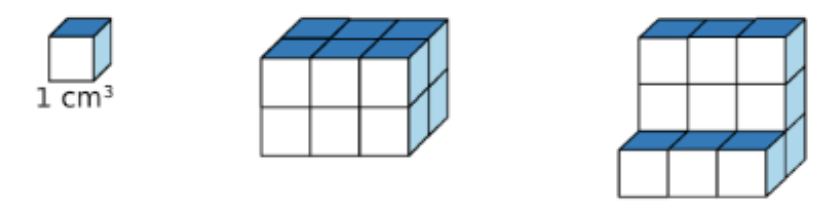
\includegraphics[scale=0.6]{IMG/4}
\end{center}

\ligne

\end{Exemple}